\chapter{Git e Github}
\label{app:git}
O Git é uma ferramenta de versionamento de código, ou seja, uma ferramenta utilizada para que toda a alteração que alguém fizer em um código tenha a possibilidade de ser marcada, assim criando uma árvore das modificações e dando ao usuário a possibilidade de navegar entre suas alterações. A ferramenta foi criada por Linus Torvalds durante a criação de Linux, para que fosse possível manter um histórico seguro do desenvolvimento do sistema operacional. Entretanto, o Git é unicamente uma ferramenta de terminal, com o desenvolvimento da internet e os recursos gráficos sendo cada vez mais utilizados para representações, juntamente com a necessidade de algo mais acessível, nasceram várias \textit{interfaces} para a ferramenta, uma delas e também a maior, o GitHub ganhou visibilidade e é hoje uma das maiores plataformas de código aberta do mundo e recentemente foi adquirida pela Microsoft\footnote{\url{https://g1.globo.com/economia/tecnologia/noticia/microsoft-compra-github-por-us-75-bilhoes.ghtml}}.

É importante saber sobre Git nos dias de hoje, maiores informações podem ser obtidas em um livro\footnote{\url{https://git-scm.com/book/en/v2}} fornecido pela própria mantenedora da ferramenta. No caso desse trabalho é possível simplesmente baixar o código pelo Github. Para isso, é necessário entender a \textit{interface} do GitHub.

Ao observar a Figura \ref{fig:git_init}, pode-se notar um cabeçalho com alguns menus, logo abaixo o nome da organização getdumont seguida pelo nome do repositório\footnote{Repositório é o nome dado ao local onde ficará armazenado todo o código de um determinado projeto}. Acessando o repositório principal do Dumont\footnote{\url{https://github.com/getdumont/dumont}} pode-se notar 5 abas, que nesse momento são irrelevantes, seguindo encontra-se alguns dados como descrição, algumas estatísticas e por fim o botão verde \textit{Clone or Download}, aqui pode-se baixar o código clicando no botão e em seguida clicando em \textit{Download ZIP}. Além disso, logo abaixo é possível ver uma tabela com a estrutura do projeto, essa estrutura é navegável pelo browser, assim qualquer arquivo citado durante essa documentação pode ser acessado sem necessidade do código na máquina.

\begin{figure}[!ht]
    \centering
    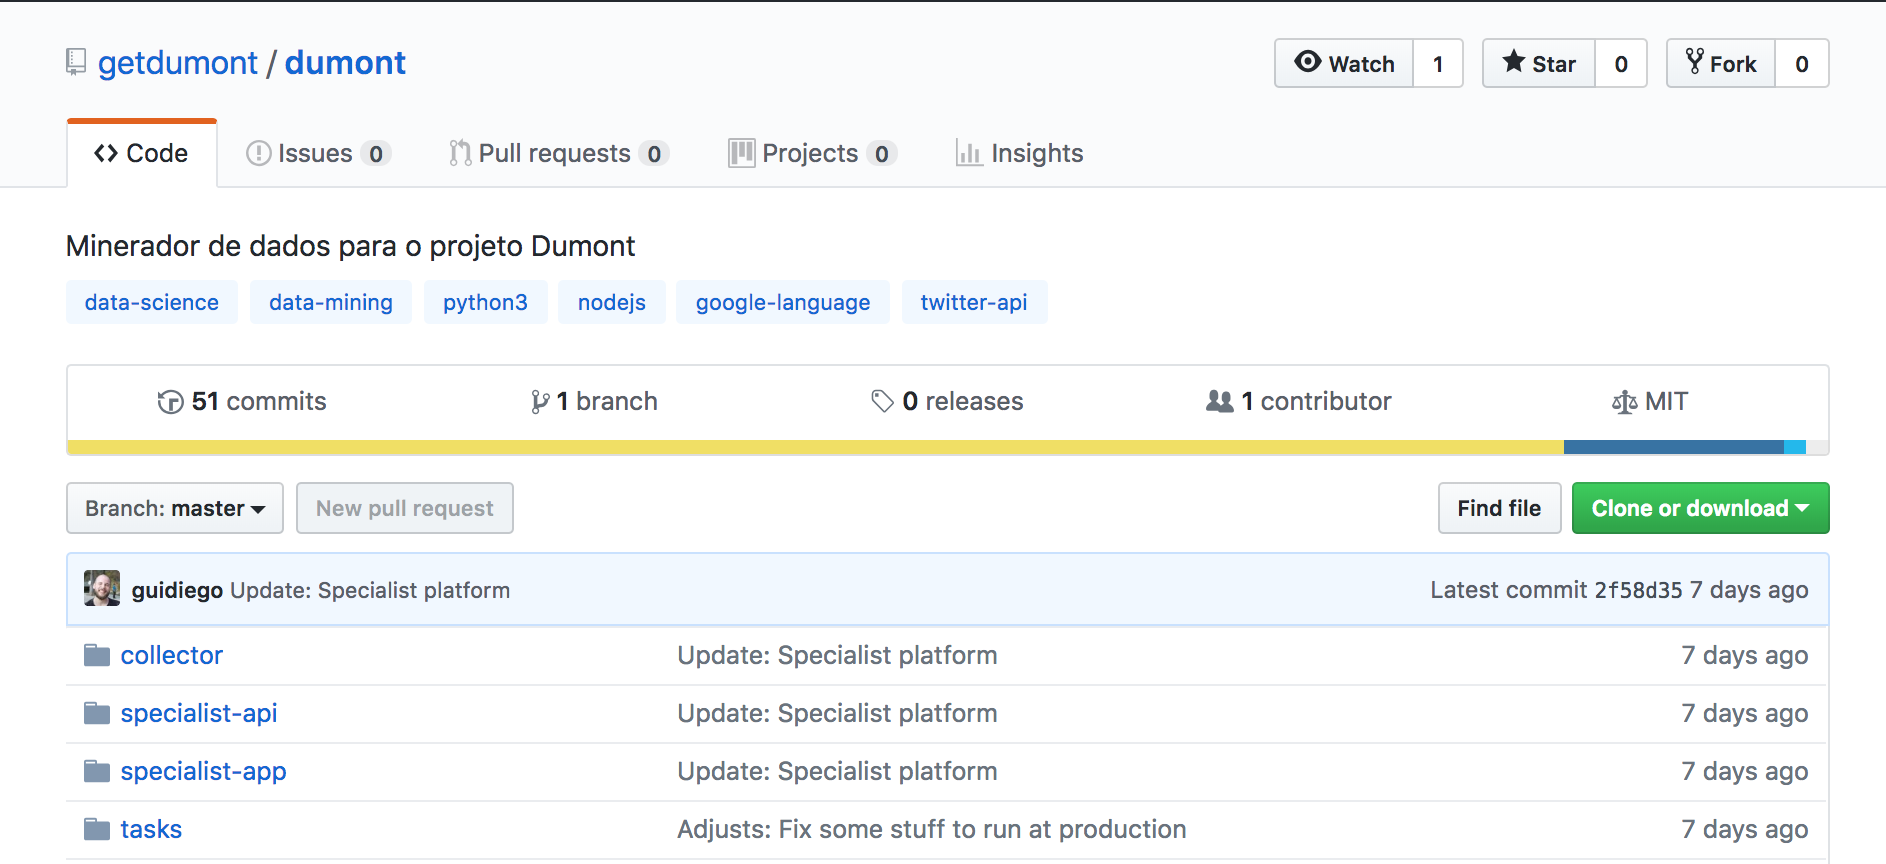
\includegraphics[width=.75\textwidth]{imagens/git_init.png}
    \caption{Imagem demonstrando a interface inicial do git}
    \label{fig:git_init}
\end{figure}

Já na Figura \ref{fig:git_file}, pode-se observar um exemplo do que foi dito anteriormente. Aqui uma demonstração de como fica um dos arquivos do projeto aberto no navegador. As 2 coisas mais importantes a serem notadas aqui é o caminho do arquivo \textit{dumont/collector/index.js} e as linhas que são mostradas no arquivo. Será utilizado destes recursos durante a documentação para exemplificar e apontar códigos.

\begin{figure}[!ht]
    \centering
    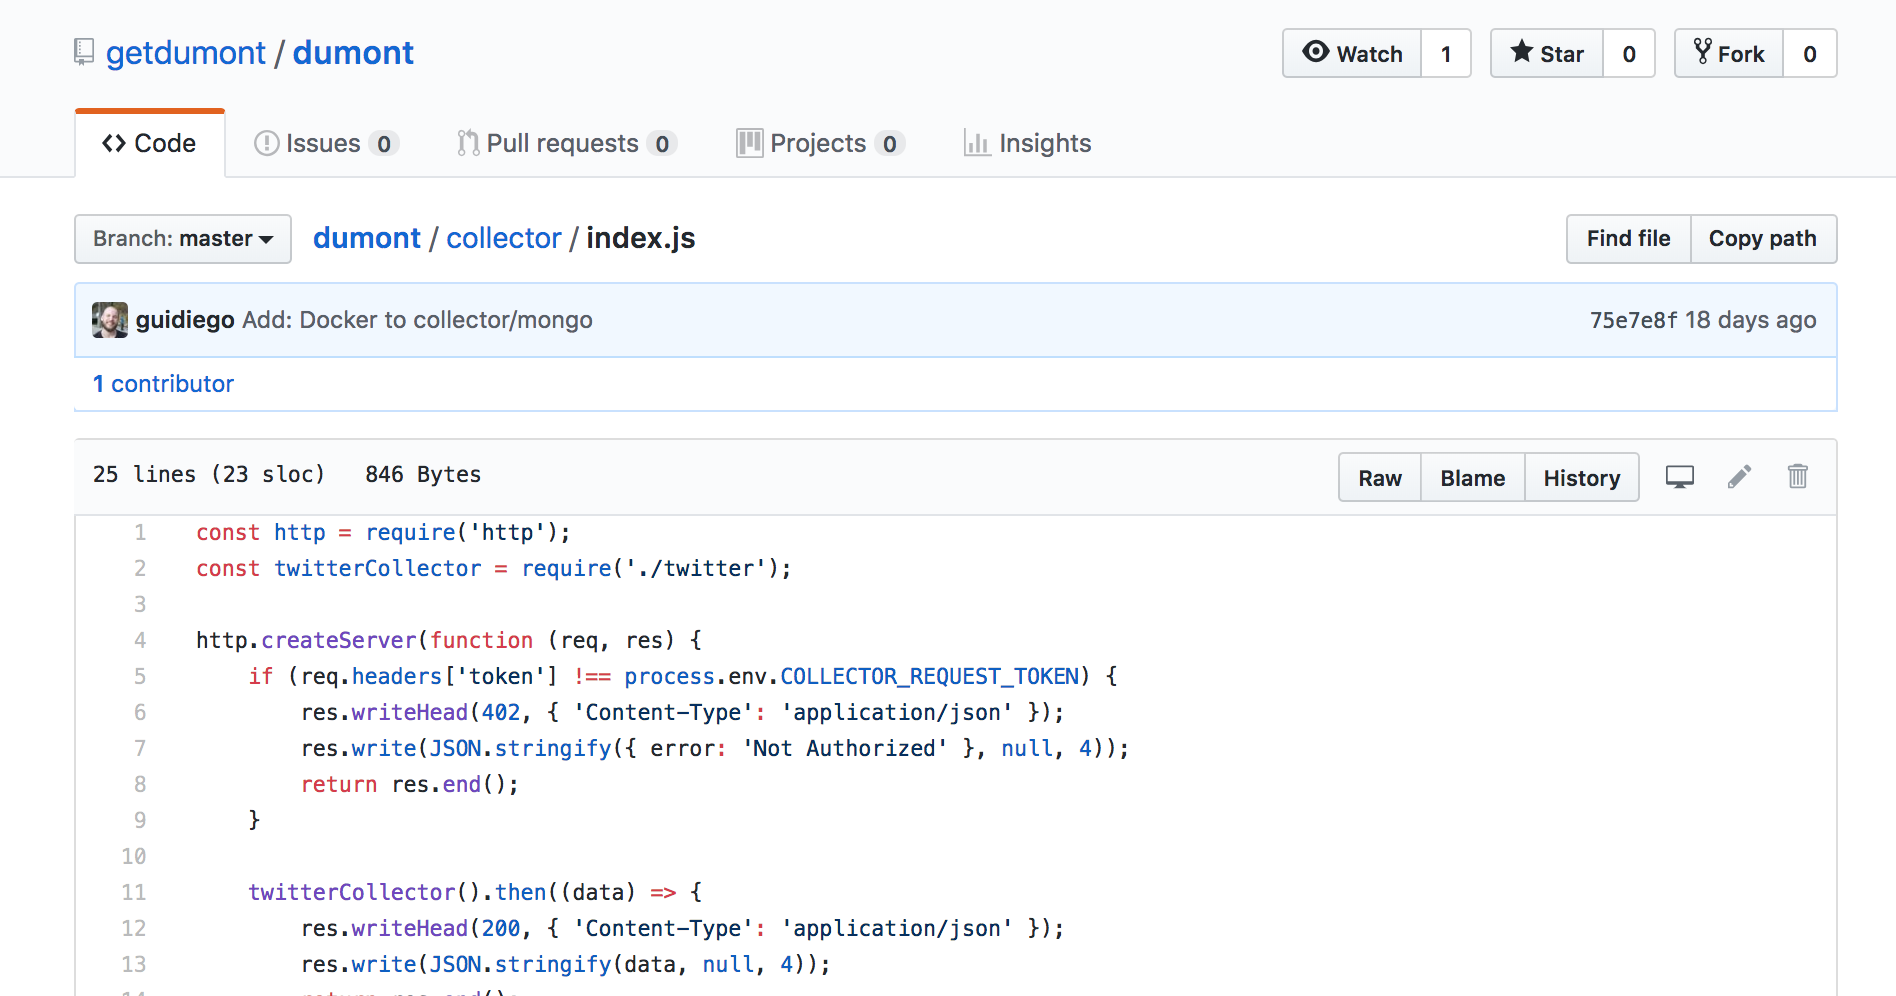
\includegraphics[width=.8\textwidth]{imagens/git_file.png}
    \caption{Imagem demonstrando a interface do git referente a um arquivo do projeto}
    \label{fig:git_file}
\end{figure}
